\section{Specific requirements}

\subsection{External interfaces}
%----------------------------------------------------------------------
\begin{tabular}{ll}
%--------------------------------
\textbf{Found in requirement}&Add User Account : FRQ1\\
\textbf{Name of item}&User name\\
\textbf{Description of purpose}&The desired User name which a user inputs\\
\textbf{Source of input}&User\\
\textbf{Destination of output}&N/A\\
\textbf{Valid range, accuracy, and/or tolerance}&Standard GSM 03.38 character set.\\
\textbf{Relationships to other inputs/outputs}&A User Account will have the User name \\&associated with it set to the inputed value.\\
&\\
&\\
%--------------------------------
\textbf{Found in requirement}&Add User Account : FRQ1\\
\textbf{Name of item}&Password\\
\textbf{Description of purpose}&The desired password which will be associated\\& with the specific user account which is being\\& created\\
\textbf{Source of input}&User\\
\textbf{Destination of output}&N/A\\
\textbf{Valid range, accuracy, and/or tolerance}&Standard GSM 03.38 character set.\\
\textbf{Relationships to other inputs/outputs}&A User Account will have the password\\& associated with it set to this value.\\
&\\
&\\
%--------------------------------
\textbf{Found in requirement}&Add User Account : FRQ1\\
\textbf{Name of item}&Password Confirmation\\
\textbf{Description of purpose}&A copy of the password to verify \\&correctness\\
\textbf{Source of input}&User\\
\textbf{Destination of output}&N/A\\
\textbf{Valid range, accuracy, and/or tolerance}&Standard GSM 03.38 character set.\\
\textbf{Relationships to other inputs/outputs}&Value submitted is used to confirm the correctness of the desired password to avoid\\& human error.\\
&\\
&\\
%--------------------------------
\textbf{Found in requirement}&Add User Account : FRQ1\\
\textbf{Name of item}&The created user account\\
\textbf{Description of purpose}&The user account that has been\\& created and has its Username and Password values set to\\& those which were defined during the account creation process \\
\textbf{Source of input}&N/A\\
\textbf{Destination of output}&Account is stored in an encrypted database\\
\textbf{Valid range, accuracy, and/or tolerance}&N/A.\\
\textbf{Relationships to other inputs/outputs}&The username and password\\& which was defined by the user is used to make the account.\\
&\\
&\\
%--------------------------------
\end{tabular}
%--------------------------------
\newpage
\begin{tabular}{ll}
%--------------------------------
\textbf{Found in requirement}&Add User Account : FRQ1\\
\textbf{Name of item}&Error message\\
\textbf{Description of purpose}&The message indicates that an account was not created and the reason for not creating the account.\\
\textbf{Source of input}&N/A\\
\textbf{Destination of output}&N/A.\\
\textbf{Valid range, accuracy, and/or tolerance}&N/A.\\
\textbf{Relationships to other inputs/outputs}&The username and password \\&which was provided by the user was invalid for one or more reasons.\\
&\\
%--------------------------------
\textbf{Found in requirement}&Local Authentication : FRQ3\\
\textbf{Name of item}&Username\\
\textbf{Description of purpose}&The username associated with the account which the user whishes to log in with.\\
\textbf{Source of input}&User\\
\textbf{Destination of output}&N/A\\
\textbf{Valid range, accuracy, and/or tolerance}&Standard GSM 03.38 character set.\\
\textbf{Relationships to other inputs/outputs}&The username that was used to create the account.\\
&\\
%--------------------------------
\textbf{Found in requirement}&Local Authentication : FRQ3\\
\textbf{Name of item}&Password\\
\textbf{Description of purpose}&The password associated with the account which the user whishes to log in to the application with.\\
\textbf{Source of input}&User\\
\textbf{Destination of output}&N/A\\
\textbf{Valid range, accuracy, and/or tolerance}&Standard GSM 03.38 character set.\\
\textbf{Relationships to other inputs/outputs}&The password that was \\&input to create the account.\\
&\\
%--------------------------------
\end{tabular}
%--------------------------------
\newpage
%--------------------------------
\begin{tabular}{ll}
%--------------------------------
\textbf{Found in requirement}&Local Authentication : FRQ3\\
\textbf{Name of item}&Error Message\\
\textbf{Description of purpose}&The error message informs the user that the authentication process failed\\
\textbf{Source of input}&N/A\\
\textbf{Destination of output}&N/A\
\textbf{Valid range, accuracy, and/or tolerance}&\\
\textbf{Relationships to other inputs/outputs}&The username and password which was enterd does not corilate with any which are stored on the device.\\
&\\
%--------------------------------
\textbf{Found in requirement}&Add Contact : FRQ10\\
\textbf{Name of item}&Contact name\\
\textbf{Description of purpose}&The name a user wishes to have associated with a certain contact.\\
\textbf{Source of input}&User\\
\textbf{Destination of output}&N/A\\
\textbf{Valid range, accuracy, and/or tolerance}&\\
\textbf{Relationships to other inputs/outputs}&Values inputted in the field will be stored in the "name" field of a contact\\
&\\
%--------------------------------
\textbf{Found in requirement}&Add Contact : FRQ10\\
\textbf{Name of item}&Contact number\\
\textbf{Description of purpose}&The cellphone number a user wishes to have associated with the contact they are adding.\\
\textbf{Source of input}&User\\
\textbf{Destination of output}&N/A\\
\textbf{Valid range, accuracy, and/or tolerance}&Standard numeric values as expected in an South African mobile phone numbers\\
\textbf{Relationships to other inputs/outputs}&The values inputted in to this field will be stored under the "phone_number" field of a contact.\\
&\\
%--------------------------------
\subsubsection{Is the local key generated by the applcation for the contact which you are adding?}
\textbf{Found in requirement}&Add Contact : FRQ10\\
\textbf{Name of item}&Local key\\
\textbf{Description of purpose}&The local key of the user for the contact.\\
\textbf{Source of input}&Application\\
\textbf{Destination of output}&N/A\\
\textbf{Valid range, accuracy, and/or tolerance}&\\
\textbf{Relationships to other inputs/outputs}&All other contact details.\\
&\\
%--------------------------------
\end{tabular}
%--------------------------------
\newpage
%--------------------------------
\begin{tabular}{ll}
%--------------------------------
\textbf{Found in requirement}&Add Contact : FRQ10\\
\textbf{Name of item}&Contact's key\\
\textbf{Description of purpose}&The contact's key which the user wishes to be associated with the specific contact he is adding adding.\\
\textbf{Source of input}&Contact\\
\textbf{Destination of output}&N/A\\
\textbf{Valid range, accuracy, and/or tolerance}&Standard GSM 03.38 character set.\\
\textbf{Relationships to other inputs/outputs}&All other contact details.\\
&\\
%--------------------------------
\textbf{Found in requirement}&Add Contact : FRQ10\\
\textbf{Name of item}&Contact\\
\textbf{Description of purpose}&The contact that was created.\\
\textbf{Source of input}&N/A\\
\textbf{Destination of output}&Local database\\
\textbf{Valid range, accuracy, and/or tolerance}&\\
\textbf{Relationships to other inputs/outputs}&All entered contact details are validated and stored in the applciations local database.\\
&\\
%--------------------------------
\textbf{Found in requirement}&Add Contact : FRQ10\\
\textbf{Name of item}&Error Message\\
\textbf{Description of purpose}&The error message informs that the contact could not be added.\\
\textbf{Source of input}&N/A\\
\textbf{Destination of output}&N/A\\
\textbf{Valid range, accuracy, and/or tolerance}&N/A\\
\textbf{Relationships to other inputs/outputs}&The contact details which the user entered were invalid.\\
&\\
%--------------------------------
\textbf{Found in requirement}&Edit Contact : FRQ11\\
\textbf{Name of item}&Contact\\
\textbf{Description of purpose}&The selected contact to be edited.\\
\textbf{Source of input}&User\\
\textbf{Destination of output}&N/A\\
\textbf{Valid range, accuracy, and/or tolerance}&\\
\textbf{Relationships to other inputs/outputs}&The contact details associated with the contact which the user selected\\
&\\
%--------------------------------
\end{tabular}
%--------------------------------
\newpage
%--------------------------------
\begin{tabular}{ll}
%--------------------------------
\textbf{Found in requirement}&Edit Contact : FRQ11\\
\textbf{Name of item}&Local key\\
\textbf{Description of purpose}&The local key of the user for the contact.\\
\textbf{Source of input}&User\\
\textbf{Destination of output}&N/A\\
\textbf{Valid range, accuracy, and/or tolerance}&\\
\textbf{Relationships to other inputs/outputs}&All other contact details.\\
&\\
%--------------------------------
\textbf{Found in requirement}&Edit Contact : FRQ11\\
\textbf{Name of item}&Contact's key\\
\textbf{Description of purpose}&The local key of the contact to be added.\\
\textbf{Source of input}&User\\
\textbf{Destination of output}&N/A\\
\textbf{Valid range, accuracy, and/or tolerance}&\\
\textbf{Relationships to other inputs/outputs}&All other contact details.\\
&\\
%--------------------------------
\textbf{Found in requirement}&Edit Contact : FRQ11\\
\textbf{Name of item}&Contact\\
\textbf{Description of purpose}&The contact that was updated.\\
\textbf{Source of input}&N/A\\
\textbf{Destination of output}&Local database\\
\textbf{Valid range, accuracy, and/or tolerance}&\\
\textbf{Relationships to other inputs/outputs}&All entered contact details.\\
&\\
%--------------------------------
\textbf{Found in requirement}&Edit Contact : FRQ11\\
\textbf{Name of item}&Error Message\\
\textbf{Description of purpose}&The error message informs the user that \\&the contact could not be edited.\\
\textbf{Source of input}&N/A\\
\textbf{Destination of output}&N/A\\
\textbf{Valid range, accuracy, and/or tolerance}&N/A\\
\textbf{Relationships to other inputs/outputs}&The contact details which were entered by the user were invalid.\\
&\\
%--------------------------------
\end{tabular}
%--------------------------------
%----------------------------------------------------------------------

\subsection{Functions}
\subsubsection{Admin Functions}
\begin{itemize}
\item{Add User Account : FRQ1}\\
\textbf{(Source: Bernard Wagner, Priority: Medium)}
\begin{itemize}
\item A user must be able to create a password protected account for the app.
\item \textbf{Inputs:} The user inputs a desired user name , password and fills in the password conformation field.
\item \textbf{Outputs:} A user account is either created and stored or an error message is displayed and no account is created.
\end{itemize}
 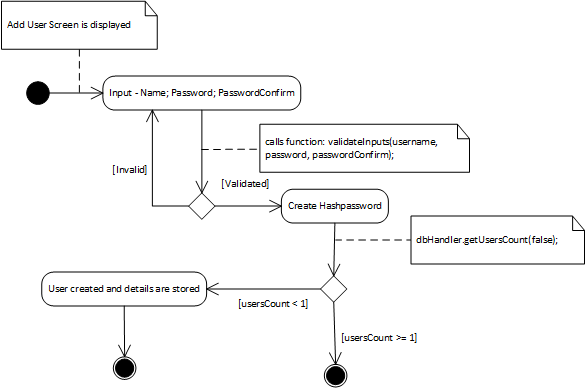
\includegraphics[width=13cm]{diagrams/StateDiagrams/AddUserStateDiagram.png}
\item{Edit User Account : FRQ2}\\
\textbf{(Source: Group Deliberation, Priority: Medium)}
\begin{itemize}
\item The user must be able to edit his/her authentication details.
\end{itemize}
 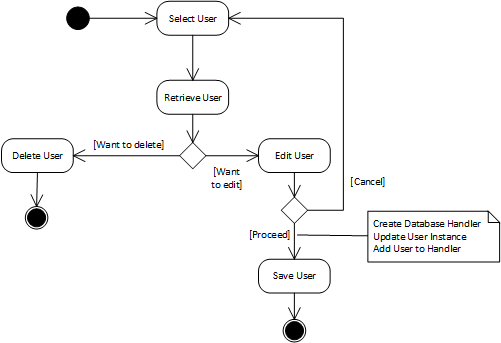
\includegraphics[width=13cm]{diagrams/StateDiagrams/EditUserStateDiagram.png}
\item{Local Authentication : FRQ3}\\%meaning functional requirement 3
\textbf{(Source: Bernard Wagner, Priority: Medium)}
\begin{itemize}
\item The application must authenticate a user by requiring a password in order to log into the application, in order to ensure confidentiality.
\item \textbf{Inputs:} The user inputs his account username and password.
\item \textbf{Outputs:} After the application has checked the users details against the stored details under that username, it will log the user in and show them the main menu or it will display an error message and refuse the inputed details.
\end{itemize}
 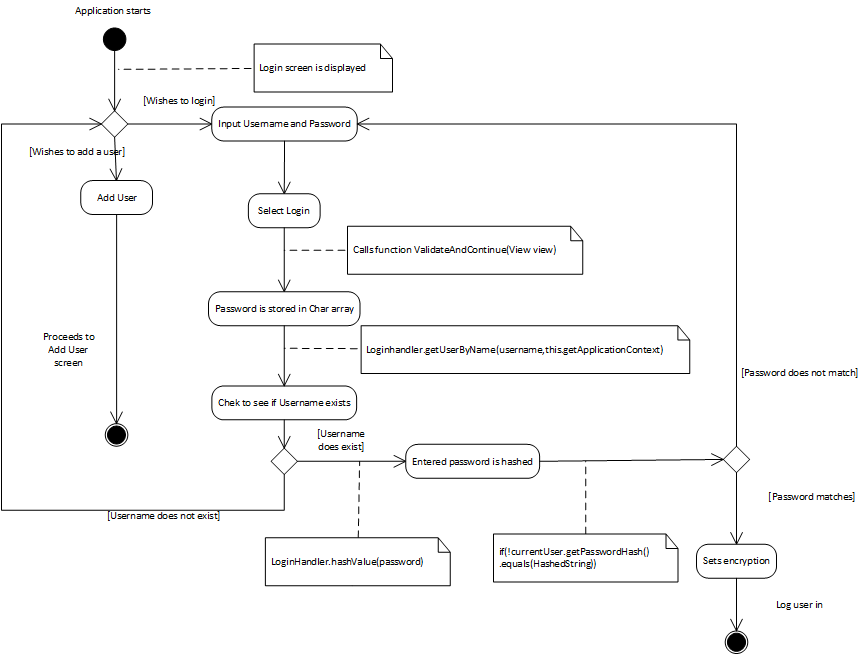
\includegraphics[width=13cm]{diagrams/StateDiagrams/LocalAuthenticationStateDiagram.png}
\end{itemize}
\subsubsection{Messaging Functions}
\begin{itemize}
\item{Enter message : FRQ4}\\%meaning functional requirement 1
\textbf{(Source: Bernard Wagner, Priority: High)}
\begin{itemize}
\item A user must be able to input text into the application.
\end{itemize}
 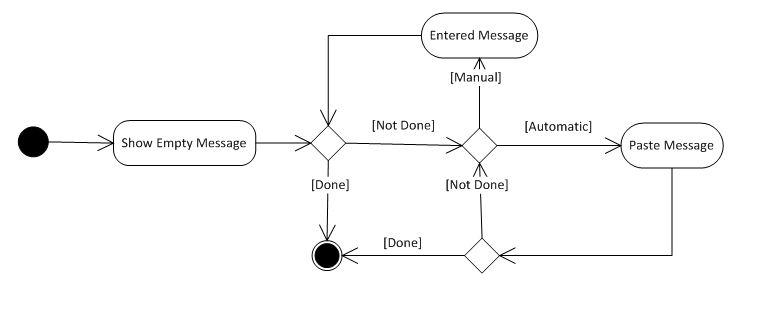
\includegraphics[width=13cm]{diagrams/StateDiagrams/EnterMessageState.png}
\item{Type message : FRQ4.1}\\
\textbf{(Source: Bernard Wagner, Priority: High)}
\begin{itemize}
\item A user must be able to type text into the application.
\end{itemize}
\item{Paste message : FRQ4.2}\\
\textbf{(Source: Bernard Wagner, Priority: High)}
\begin{itemize}
\item A user must be able to paste an already constructed message into the application, using the clipboard.
\end{itemize}
\item{Edit Message: FRQ5}\\
\textbf{(Source: Bernard Wagner, Priority: Medium)}
\begin{itemize}
\item The message text must be editable once it has been input into the application by the user.
\end{itemize}
 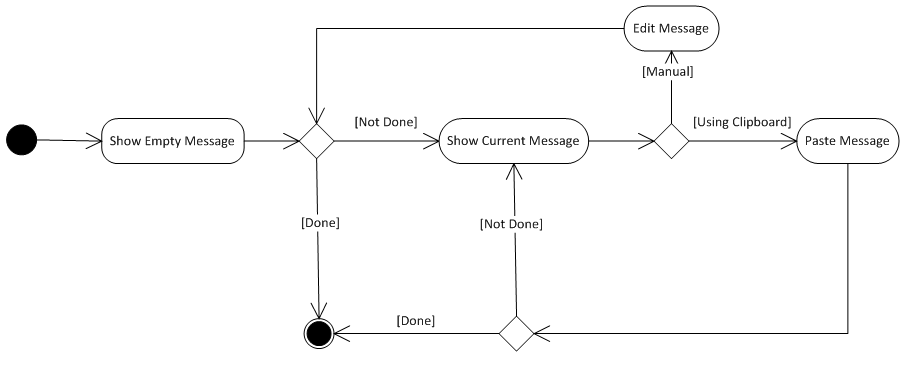
\includegraphics[width=13cm]{diagrams/StateDiagrams/EditMessageState.png}
\item{Encrypt message : FRQ6}\\
\textbf{(Source: Bernard Wagner, Priority: High)}
\begin{itemize}
\item The message must be encrypted using a suitable encryption method.
\end{itemize}
 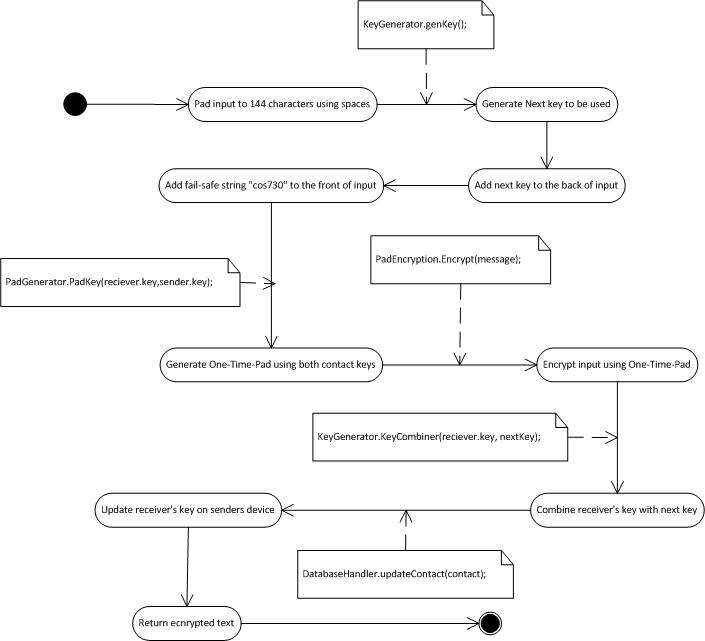
\includegraphics[width=13cm]{diagrams/StateDiagrams/EncryptMessageStateDiagram.png}
\item{Copy Encrypted Message : FRQ7}\\
\textbf{(Source: Bernard Wagner, Priority: High)}
\begin{itemize}
\item Once a message has been encrypted, a user must be able to copy the ciphertext, and paste it into a suitable messaging application.
\end{itemize}
\item{Decrypt message : FRQ8}\\
\textbf{(Source: Bernard Wagner, Priority: High)}
\begin{itemize}
\item The application must be able to decrypt the message (on the receiving end) to reveal the original text.
\end{itemize}
 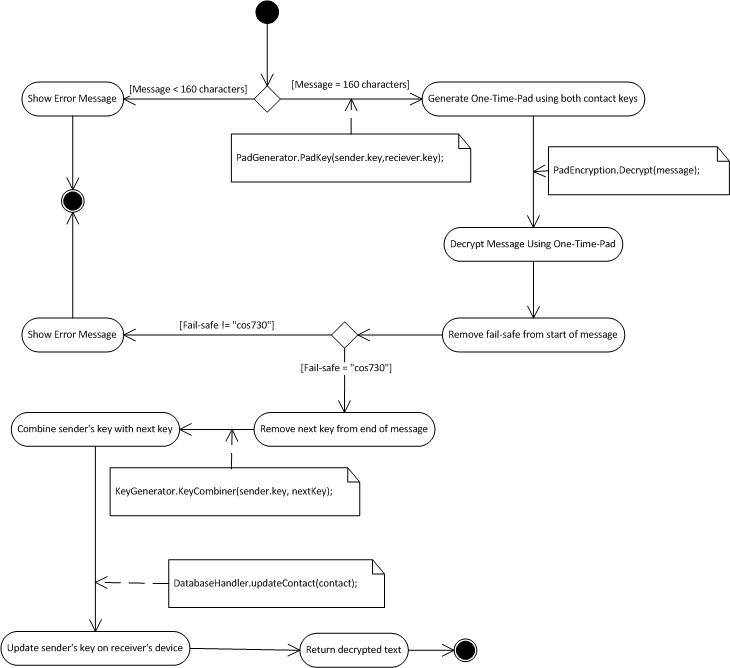
\includegraphics[width=13cm]{diagrams/StateDiagrams/DecryptMessageStateDiagram.png}
\item{Display message length : FRQ9}\\
\textbf{(Source: Bernard Wagner, Priority: Low)}
\begin{itemize}
\item The numbers of characters in the message must be displayed.
\end{itemize}
 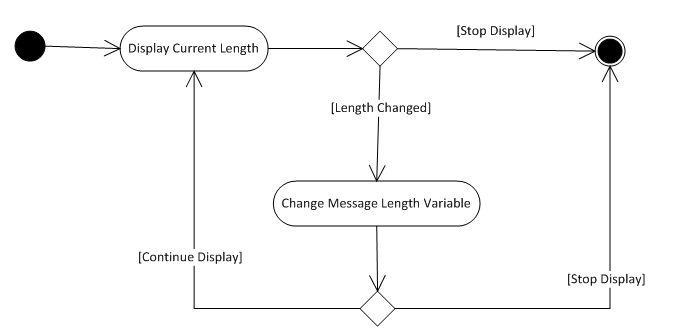
\includegraphics[width=13cm]{diagrams/StateDiagrams/DisplayMessageLengthState.png}
\end{itemize}
\subsubsection{Contacts Functions}
\begin{itemize}
\item{Add Contact : FRQ10}\\
\textbf{(Source: Bernard Wagner, Priority: High)}
\begin{itemize}
\item Before communicating with someone, the receiver must be added as a contact, in order to be able to communicate with that user.
\item \textbf{Inputs:} The user inputs a contact's Name,number,local key and the contacts key.
\item \textbf{Outputs:} The contact is created and stored or the apllication shows an error message if input details were invalid.
\end{itemize}
 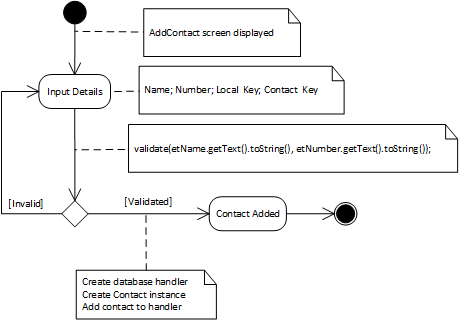
\includegraphics[width=13cm]{diagrams/StateDiagrams/AddContactStateDiagram.png}
\item{Edit Contact : FRQ11}\\
\textbf{(Source: Bernard Wagner, Priority: Medium)}
\begin{itemize}
\item A contact must be editable once it has been added.
\item \textbf{Inputs:} The user selects a contact which they wish to modify the details for or to delete from the application.
\item \textbf{Outputs:} The selected contacts details will be modified and stored or the contact will be deleted.
\end{itemize}
 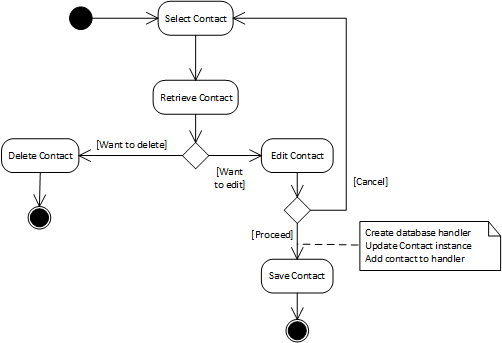
\includegraphics[width=13cm]{diagrams/StateDiagrams/EditContactStateDiagram.png}
\item{Synchronise Contact : FRQ12}\\
\textbf{(Source: Group Deliberation, Priority: High)}
\begin{itemize}
\item The user shall be able to synchronise with a contact at any time after they have been added.
\end{itemize}
 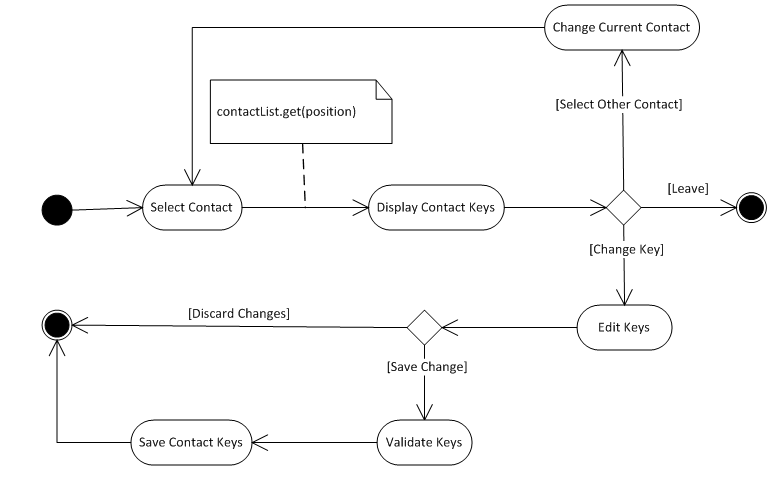
\includegraphics[width=13cm]{diagrams/StateDiagrams/SynchroniseContactState.png}
\item{Remove Contact : FRQ13}\\
\textbf{(Source: Bernard Wagner, Priority: High)}
\begin{itemize}
\item A user must be able to remove a contact.
\end{itemize}
 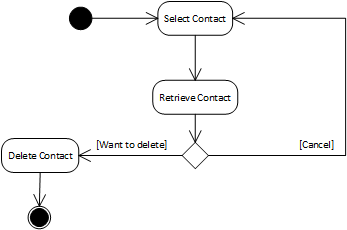
\includegraphics[width=11cm]{diagrams/StateDiagrams/RemoveContactStateDiagram.png}
\end{itemize}

\subsection{Performance requirements}
\begin{itemize}
\item The application should operate in a timely manner, the user should not be made to wait an unreasonable amount of time (this variable can be affected by the system environment e.g. resource availability).
\begin{itemize}
\item Expected time the applcaiton should take to decrypt is less than one second.
\item Expected time the applicaiton should take to encrypt is less than one second.
\end{itemize}
\item The encryption method must be secure.
\begin{itemize}
\item The Encyprion method used should have an entropy of less than 1\%.
\end{itemize}
\item The applcaiton must be secure.
\begin{itemize}
\item A user’s password must not be viewable as to prevent unauthorized use of the application.
\item A user’s password should be encrypted or stored as a hash value.
\item Contact information stored by the application must not be obtainable by unauthorized users.
\item Contact information should be encrypted to ensure that it is not readable by unauthorized users.
\end{itemize}
\end{itemize}

\subsection{Logical database requirements}

\begin{itemize}
\item The password must be hashed using a SHA-256 hash function.
\item The data should only be viewable by an authorised user.
\item The contact data must be encrypted to ensure confidentiality using an applicable hash function.
\item Every user has 0 or more contacts associated with it.
\item Once a user is deleted, all contacts are deleted along with the user.
\end{itemize}
\begin{center}
 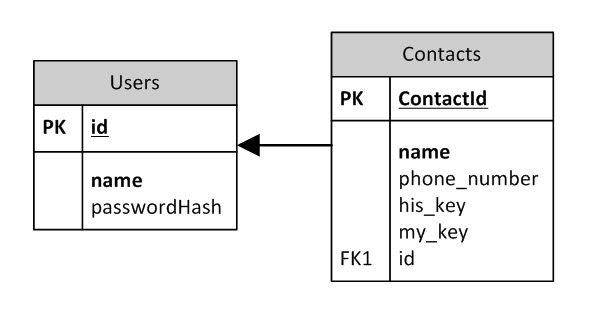
\includegraphics[width=13cm]{diagrams/LogicalDatabase.png}
\end{center}

\subsection{Design constraints}
\begin{itemize}
\item{Message length : DC1}\\
\textbf{(Source: Bernard Wagner, Priority: High)}
\begin{itemize}
\item Due to the fact that the primary messaging service which the client intends to use is SMS this limits the input size of the text to 160 characters. 
\item The encryption process uses 6 characters for a fail safe and 10 characters to embed the next key.
\item This means plaintext must be limited to 144 characters.
\item To maintain consistency we enforce this as the maximum length of messages which the application can encrypt, regardless of the intended messaging application.
\end{itemize}
\item{The usable characters : DC2}\\
\textbf{(Source: Bernard Wagner, Priority: High)}
\begin{itemize}
\item The usable character which can be encrypted by the application is the GSM character set because the primary intended messaging service that the client wishes to use is SMS. 
\end{itemize}
\item{Application resource requirementsr : DC3}\\
\textbf{(Source: Bernard Wagner, Priority: High)}
\begin{itemize}
\item The application should function efficiently with the least amount of resource usage.
\end{itemize}
\end{itemize}
\subsubsection{Standards compliance}
\begin{itemize}
\item The application must be secure, as is stipuled in Appendix D, Secure design principles.
\item The Application must conform to the Android and iOS design principles for each respective platform, these can be found in Appendix E, Design principles.
\end{itemize}

\subsection{Software system attributes}
\subsubsection{Reliability}
\begin{itemize}
\item The application should run until the user closes it.
\item Any information stored in the application should be static and exist as long as the application is open or said information is removed/edited.
\item The ciphertext should decrypt into its plaintext.
\end{itemize}
\subsubsection{Availability}
\begin{itemize}
\item The user should be able to use the application as long as it is running and should not be made to wait while the application performs a function.
\item The application should not interfere with any other applications which are running on the device.
\end{itemize}
\subsubsection{Security}
\begin{itemize}
\item A secure encryption and decryption method will be used for the localised database.
\end{itemize}
\subsubsection{Maintainability}
\begin{itemize}
\item The source code should be maintainable (simplistic and readable/documented).
\item The application should not act in unpredictable ways.
\end{itemize}
\subsubsection{Portability}
\begin{itemize}
\item The client has requested that different versions of the application be developed to execute on different operating systems namely Android and iOS.
\end{itemize}
